\documentclass[conference]{IEEEtran}
\IEEEoverridecommandlockouts

% Packages
\usepackage{cite}
\usepackage{amsmath,amssymb,amsfonts}
\usepackage{graphicx}
\usepackage{textcomp}
\usepackage{listings}
\usepackage{subcaption}
\usepackage{float}
\usepackage{multirow}
\usepackage{algorithm}
\usepackage{algpseudocode}
\usepackage{algorithmicx}
\usepackage{url}
\usepackage{caption}
\usepackage{tcolorbox}
\usepackage{hyperref}
\usepackage[T1]{fontenc}
\usepackage{enumitem}
\usepackage{multicol}
\usepackage{enumitem}
\usepackage{balance}
\usepackage{array,booktabs}

\setlength {\marginparwidth }{2cm}
\newlength{\subfigwidth}
\setlength{\subfigwidth}{0.15\textwidth}
\newcolumntype{M}[1]{>{\centering\arraybackslash}m{#1}} % w/ horizontal centering


\hypersetup{hidelinks}

\tcbuselibrary{listingsutf8}
\newtcbox{\redbox}[1][]{
 on line, 
 boxsep=1pt, 
 left=1pt, 
 right=1pt, 
 top=1pt, 
 bottom=1pt, 
 colframe=red!75!black, 
 colback=red!10, 
 boxrule=0.5pt, 
 rounded corners,
 #1
}

\algrenewcommand\algorithmicindent{0.8em} 

\begin{document}

\title{Proliferating Cell Collectives: \\A Comparison of Hard and Soft Collision Models}

\author{
    \IEEEauthorblockN{Manuel Lerchner}
    \IEEEauthorblockA{
        \textit{Technical University of Munich}\\
        Munich, Germany}
}

\maketitle

\begin{abstract}
    This thesis investigates the computational modeling of proliferating cell collectives, focusing on the fundamental differences between hard (constraint-based) and soft (potential-based) collision models. Building on recent advances in understanding bacterial colony pattern formation \cite{Weady2024}, we demonstrate that both approaches can reproduce the experimentally observed patterns. However, we show that the soft collision model faces inherent limitations in handling growth events and maintaining proper particle spacing.

\end{abstract}

\begin{IEEEkeywords}
    active matter, cell collectives, particle simulation, constraint optimization, pattern formation, computational biology
\end{IEEEkeywords}

\section{Introduction}
\subsection{Biological Motivation}
\begin{itemize}
    \item Cell collectives and pattern formation in nature
    \item Experimental observations of bacterial colony growth
    \item Importance of understanding collective behavior
\end{itemize}

\subsection{Computational Challenges}
\begin{itemize}
    \item Modeling proliferating active matter systems
    \item Trade-offs between computational efficiency and accuracy
    \item Time scale separation in growing systems
\end{itemize}

\subsection{Research Questions}
\begin{itemize}
    \item Comparison of hard vs. soft collision models
    \item Impact of model choice on pattern formation
    \item Computational performance considerations
\end{itemize}

\section{Background and Literature Review}
\subsection{Proliferating Active Matter}
\begin{itemize}
    \item Theoretical foundations of growing active matter systems
    \item Key differences from static particle systems
    \item The Weady et al. framework for pattern formation
    \item Mechanically driven growth in confined spaces
\end{itemize}

\subsection{Collision Models}
\begin{itemize}
    \item Hard collision approaches
    \item Soft collision methods
    \item Known limitations
\end{itemize}

\subsection{Cell Mechanics}
\begin{itemize}
    \item Rigid vs. deformable assumptions
    \item Experimental evidence
    \item Model selection implications
\end{itemize}

\section{Mathematical Formulations}
\subsection{Hard Collision Model}
\begin{itemize}
    \item Constraint optimization
    \item Growth dynamics
    \item Time integration
\end{itemize}

\subsection{Soft Collision Model}
\begin{itemize}
    \item Potential functions
    \item Force calculations
    \item Stability considerations
\end{itemize}

\section{Implementation and Results}
\subsection{Simulation Framework}
\begin{itemize}
    \item Implementation details
    \item Data structures
    \item Performance optimization
\end{itemize}

\subsection{Pattern Formation Analysis}


\begin{figure*}

    \centering
    \begin{subfigure}[b]{\textwidth}

        \begin{tabular}{r M{\subfigwidth} M{\subfigwidth} M{\subfigwidth} M{\subfigwidth} M{\subfigwidth} }
            Hard                                                                                    &
            \begin{subfigure}[b]{\subfigwidth}
                
\includegraphics[width=\textwidth]{figures/growth_comparison_lambda_1e-3/hard.0019.png}
            \end{subfigure} &
            \begin{subfigure}[b]{\subfigwidth}
                
\includegraphics[width=\textwidth]{figures/growth_comparison_lambda_1e-3/hard.0038.png}
            \end{subfigure} &
            \begin{subfigure}[b]{\subfigwidth}
                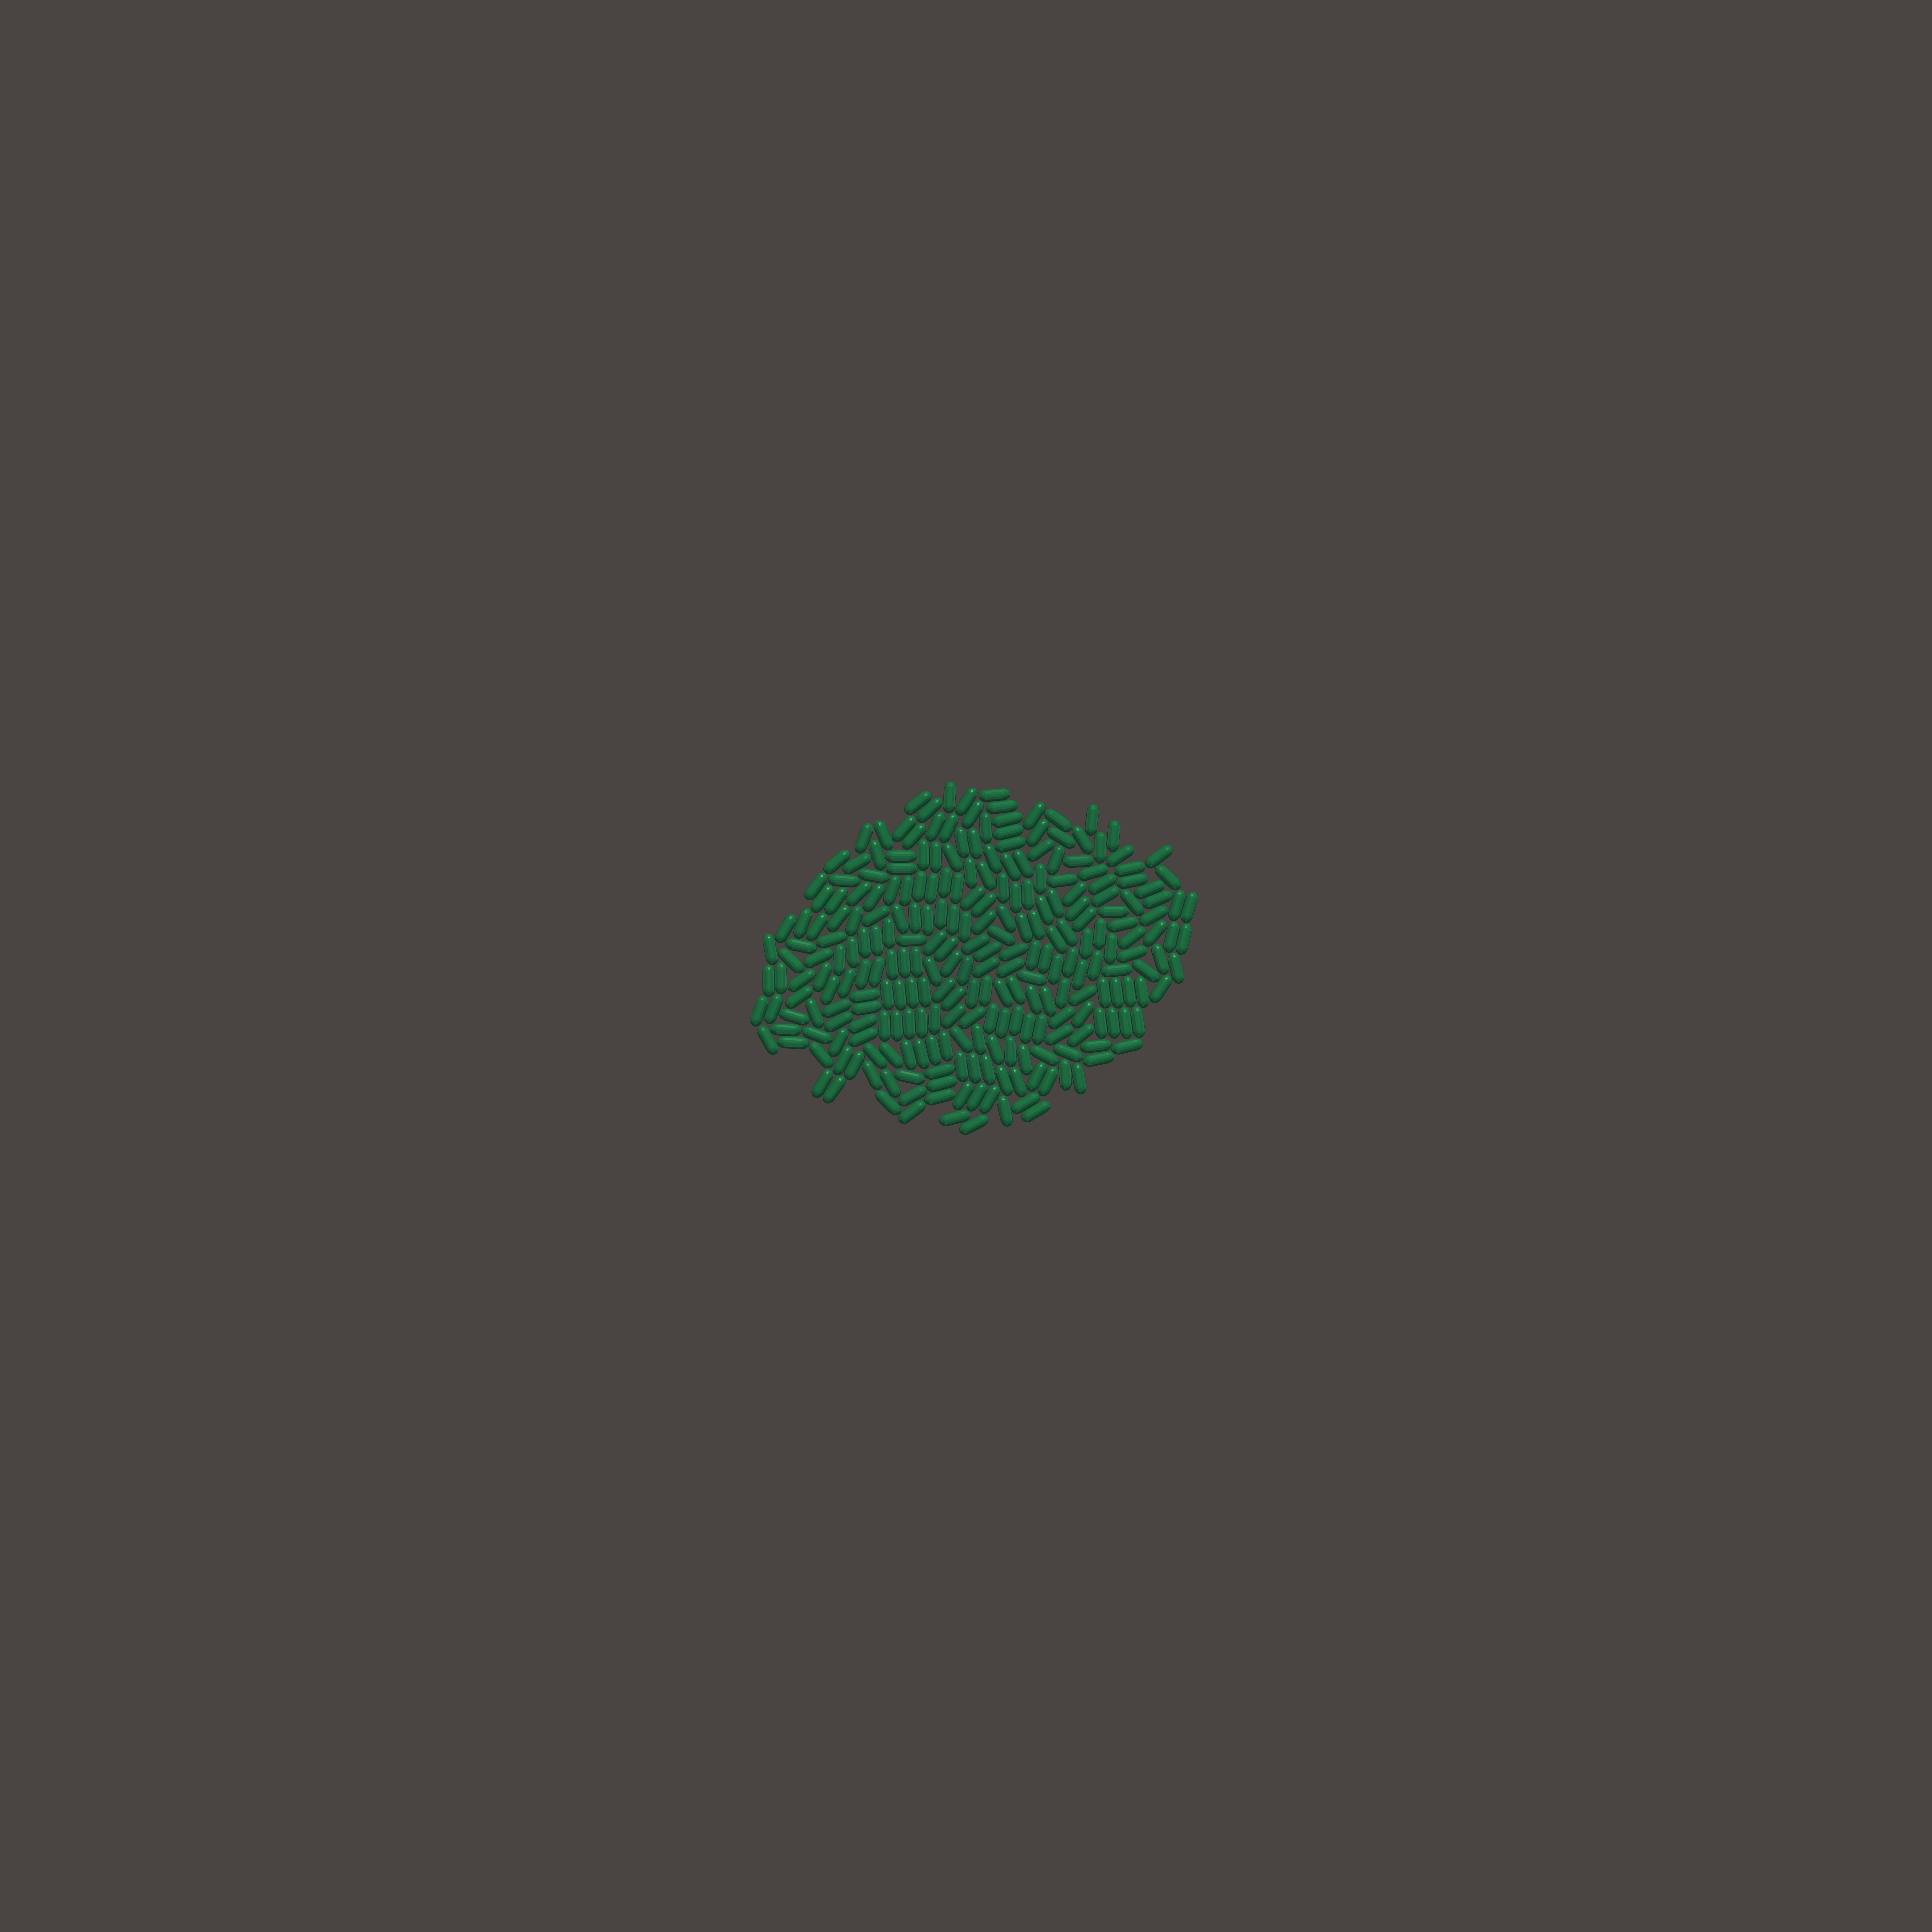
\includegraphics[width=\textwidth]{figures/growth_comparison_lambda_1e-3/hard.0057.png}
            \end{subfigure} &
            \begin{subfigure}[b]{\subfigwidth}
                \includegraphics[width=\textwidth]{figures/growth_comparison_lambda_1e-3/hard.0076.png}
            \end{subfigure} &
            \begin{subfigure}[t]{\subfigwidth}
                \includegraphics[width=\textwidth]{figures/growth_comparison_lambda_1e-3/hard.0095.png}
            \end{subfigure}    \\

            Soft                                                                                    &
            \begin{subfigure}[b]{\subfigwidth}
                
\includegraphics[width=\textwidth]{figures/growth_comparison_lambda_1e-3/soft.0019.png}
            \end{subfigure} &
            \begin{subfigure}[b]{\subfigwidth}
                
\includegraphics[width=\textwidth]{figures/growth_comparison_lambda_1e-3/soft.0035.png}
            \end{subfigure} &
            \begin{subfigure}[b]{\subfigwidth}
                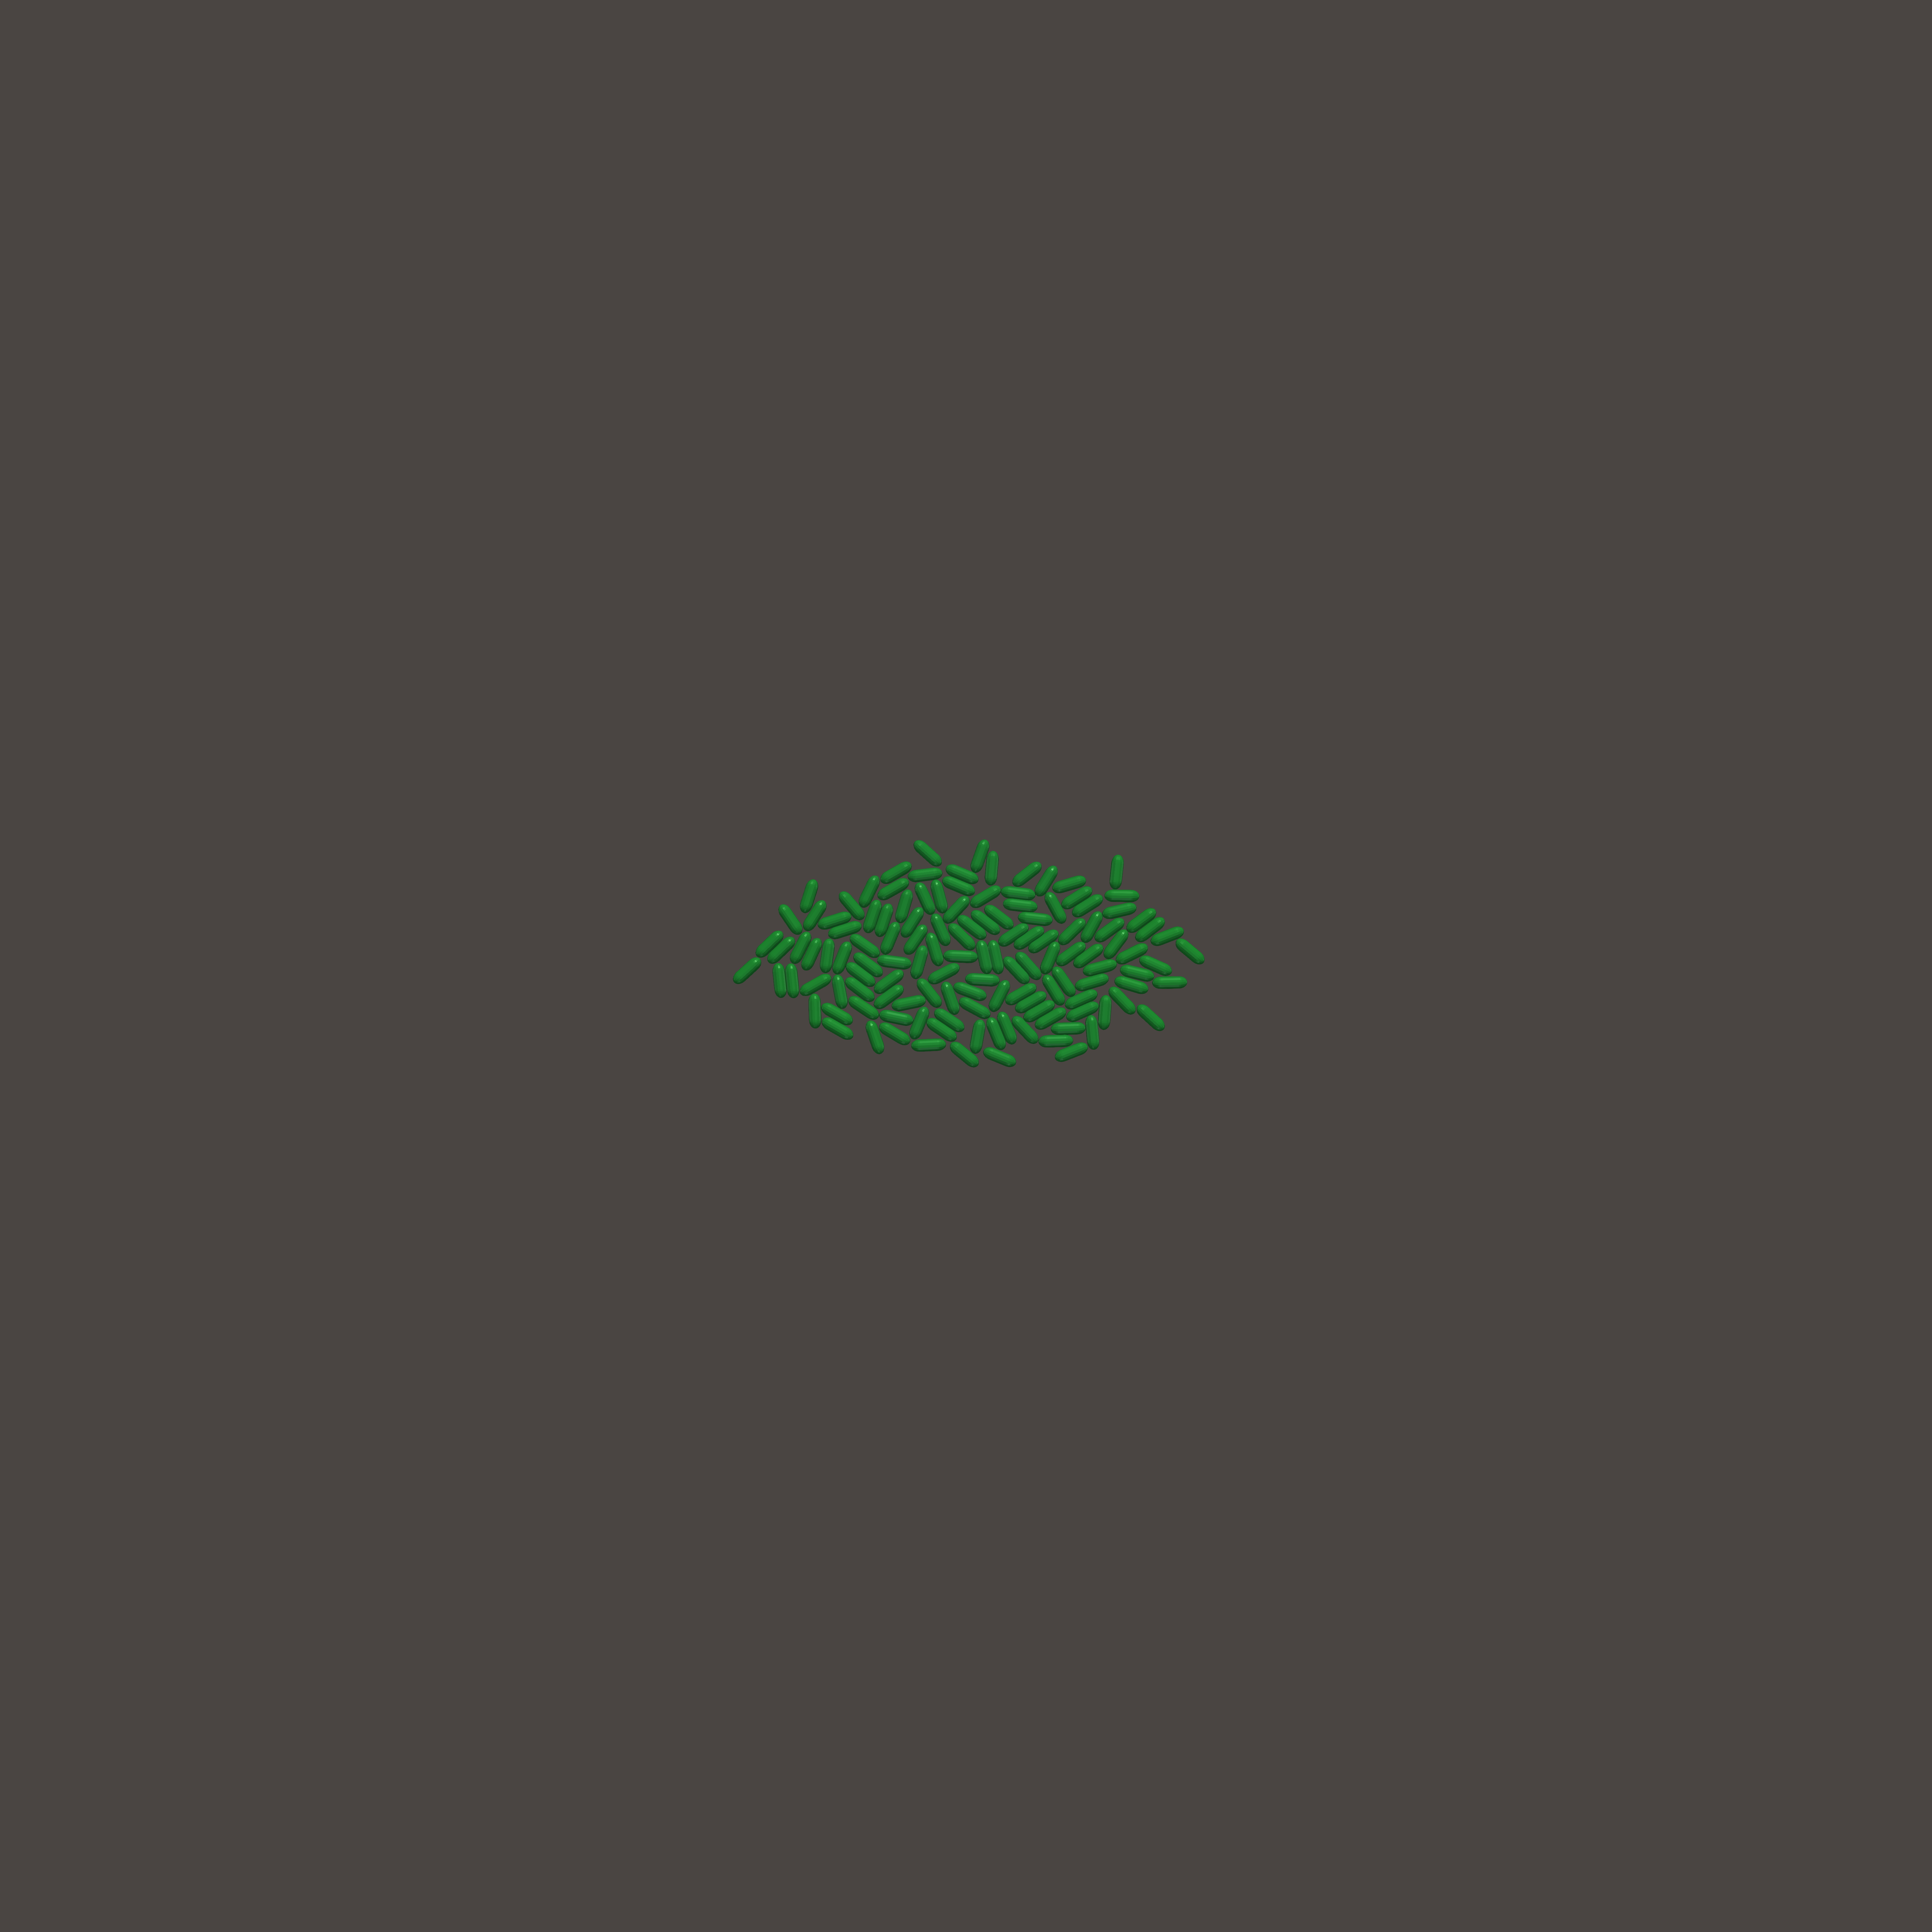
\includegraphics[width=\textwidth]{figures/growth_comparison_lambda_1e-3/soft.0051.png}
            \end{subfigure} &
            \begin{subfigure}[b]{\subfigwidth}
                \includegraphics[width=\textwidth]{figures/growth_comparison_lambda_1e-3/soft.0083.png}
            \end{subfigure} &
            \begin{subfigure}[t]{\subfigwidth}
                \includegraphics[width=\textwidth]{figures/growth_comparison_lambda_1e-3/soft.0099.png}
            \end{subfigure}    \\
        \end{tabular}
        \caption{Growth Comparison $\lambda=10^{-3}$}


    \end{subfigure}

    \vspace{1em}


    \begin{subfigure}[b]{\textwidth}

        \begin{tabular}{r M{\subfigwidth} M{\subfigwidth} M{\subfigwidth} M{\subfigwidth} M{\subfigwidth} }
            Hard                                                                                    &
            \begin{subfigure}[b]{\subfigwidth}
                
\includegraphics[width=\textwidth]{figures/growth_comparison_lambda_1e-2/hard.0020.png}
            \end{subfigure} &
            \begin{subfigure}[b]{\subfigwidth}
                
\includegraphics[width=\textwidth]{figures/growth_comparison_lambda_1e-2/hard.0040.png}
            \end{subfigure} &
            \begin{subfigure}[b]{\subfigwidth}
                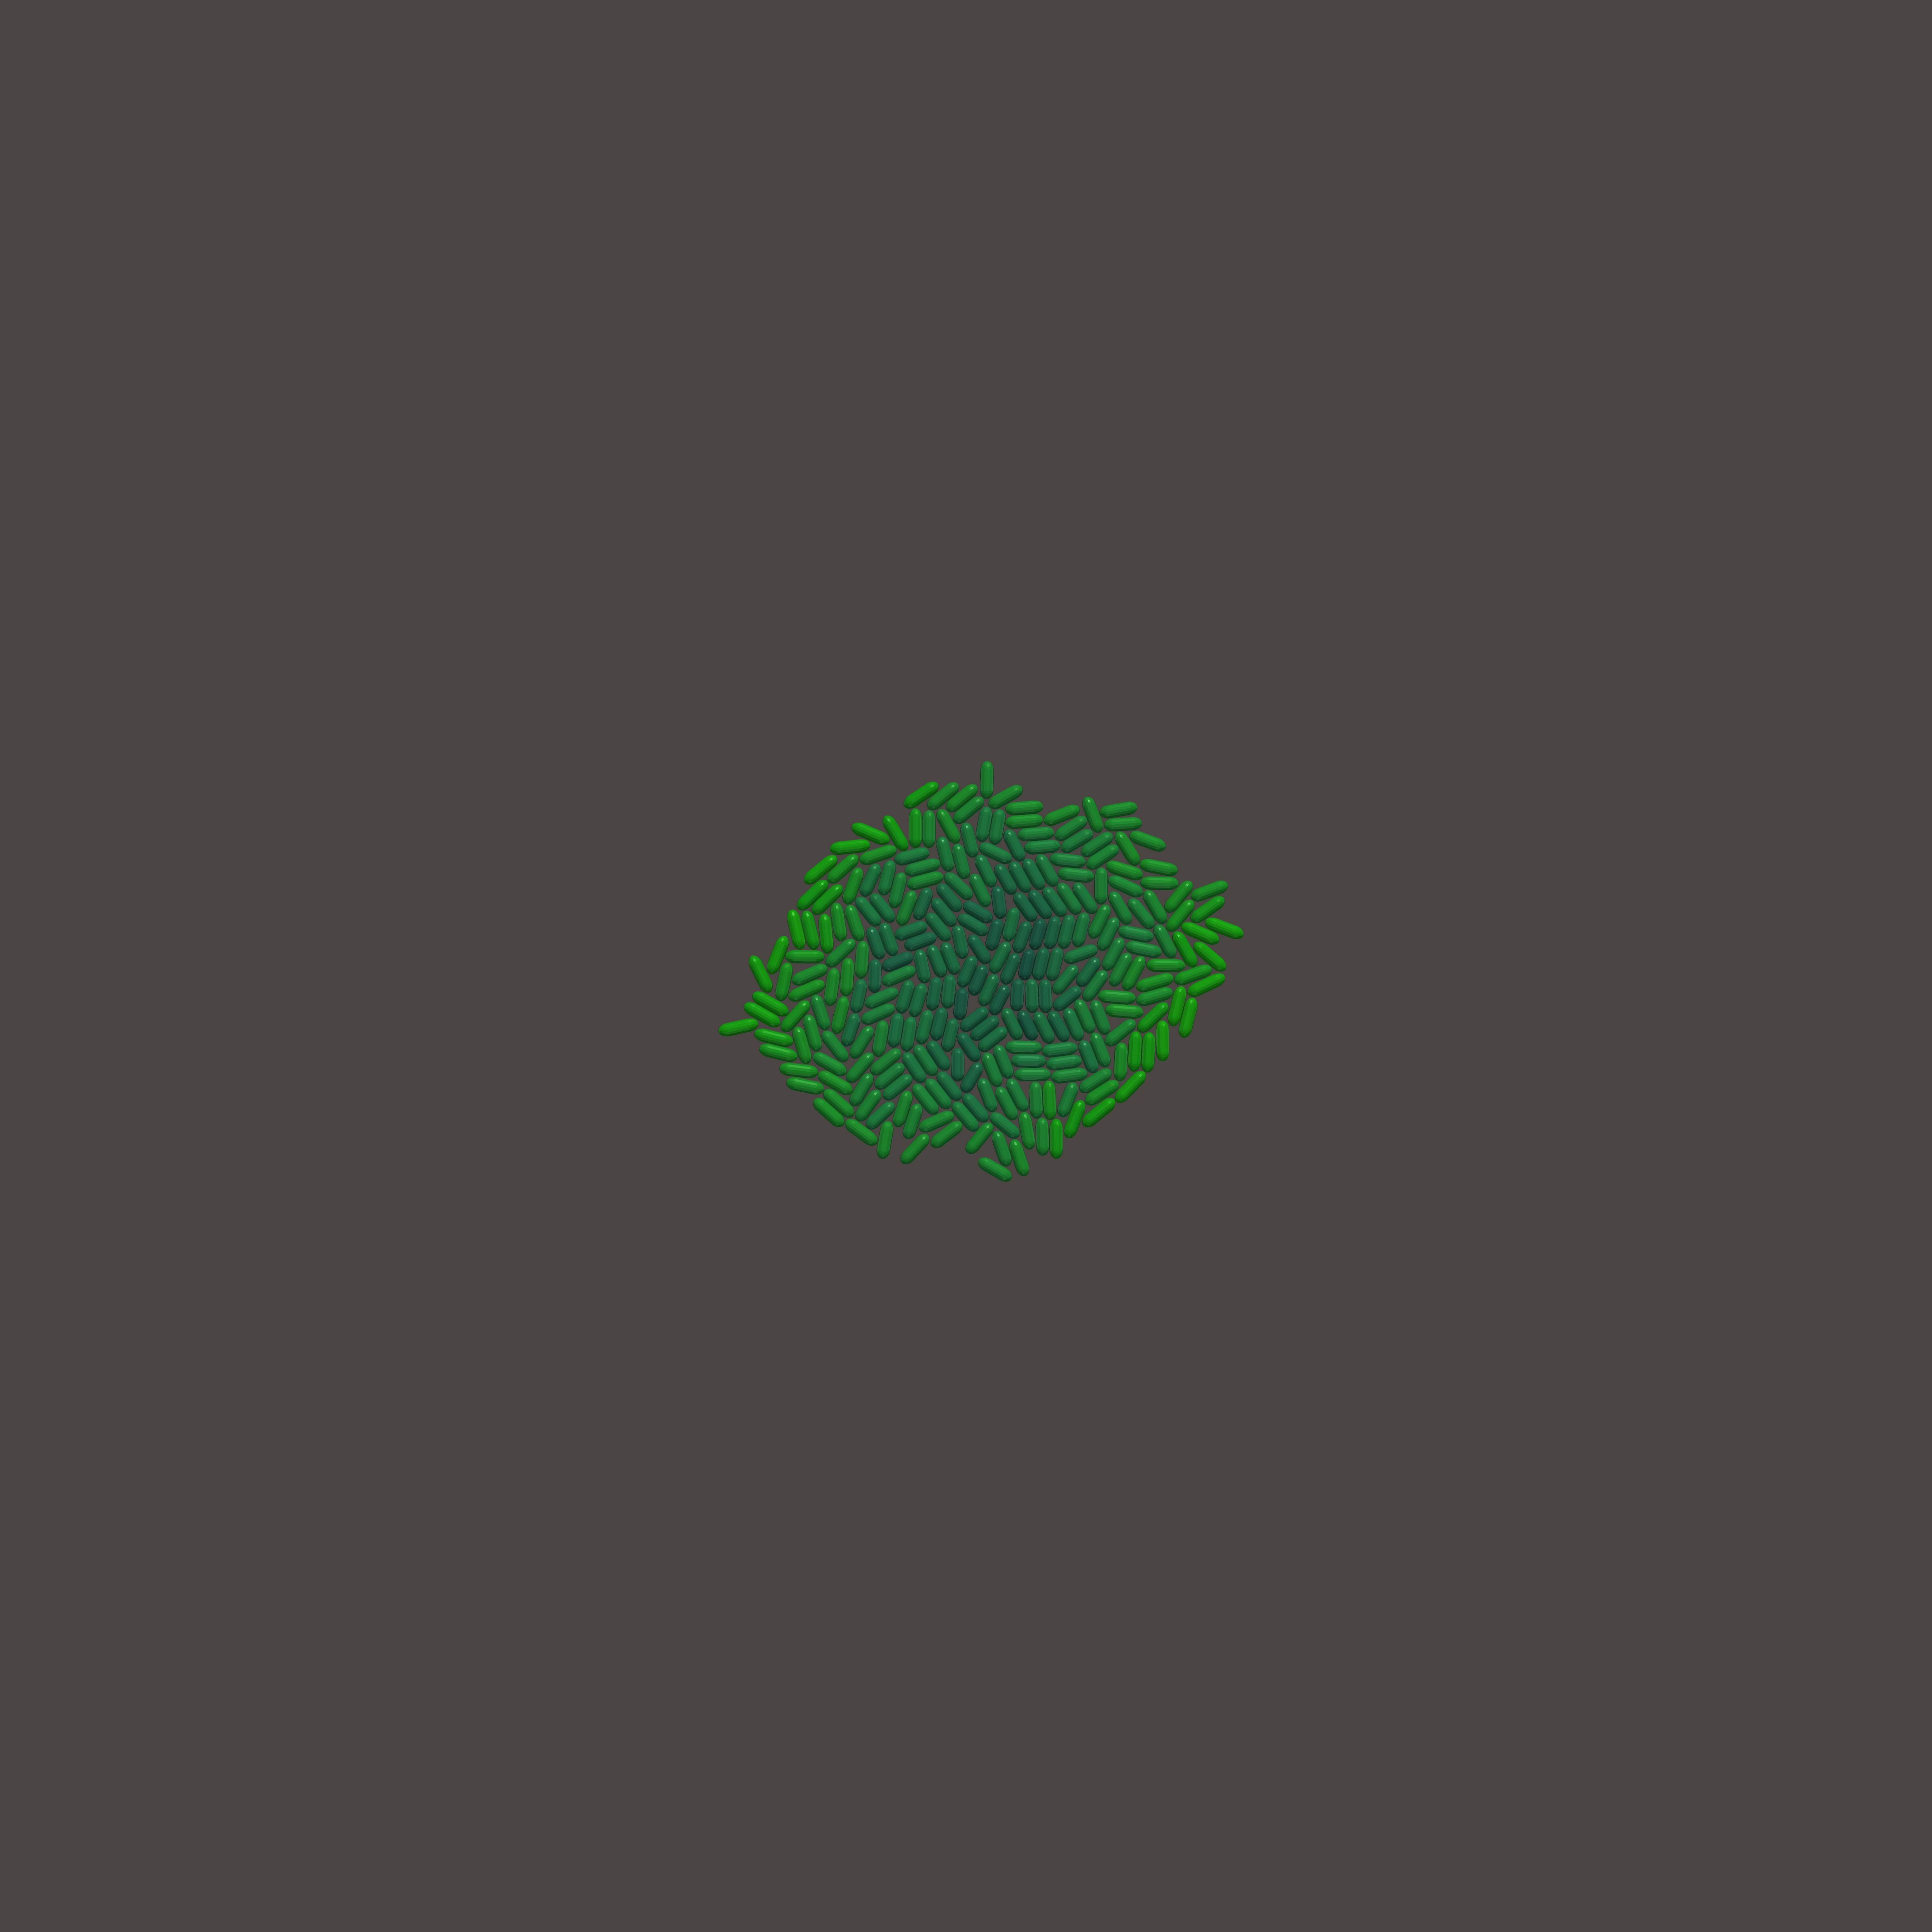
\includegraphics[width=\textwidth]{figures/growth_comparison_lambda_1e-2/hard.0060.png}
            \end{subfigure} &
            \begin{subfigure}[b]{\subfigwidth}
                \includegraphics[width=\textwidth]{figures/growth_comparison_lambda_1e-2/hard.0080.png}
            \end{subfigure} &
            \begin{subfigure}[t]{\subfigwidth}
                \includegraphics[width=\textwidth]{figures/growth_comparison_lambda_1e-2/hard.0100.png}
            \end{subfigure}    \\

            Soft                                                                                    &
            \begin{subfigure}[b]{\subfigwidth}
                
\includegraphics[width=\textwidth]{figures/growth_comparison_lambda_1e-2/soft.0020.png}
            \end{subfigure} &
            \begin{subfigure}[b]{\subfigwidth}
                
\includegraphics[width=\textwidth]{figures/growth_comparison_lambda_1e-2/soft.0040.png}
            \end{subfigure} &
            \begin{subfigure}[b]{\subfigwidth}
                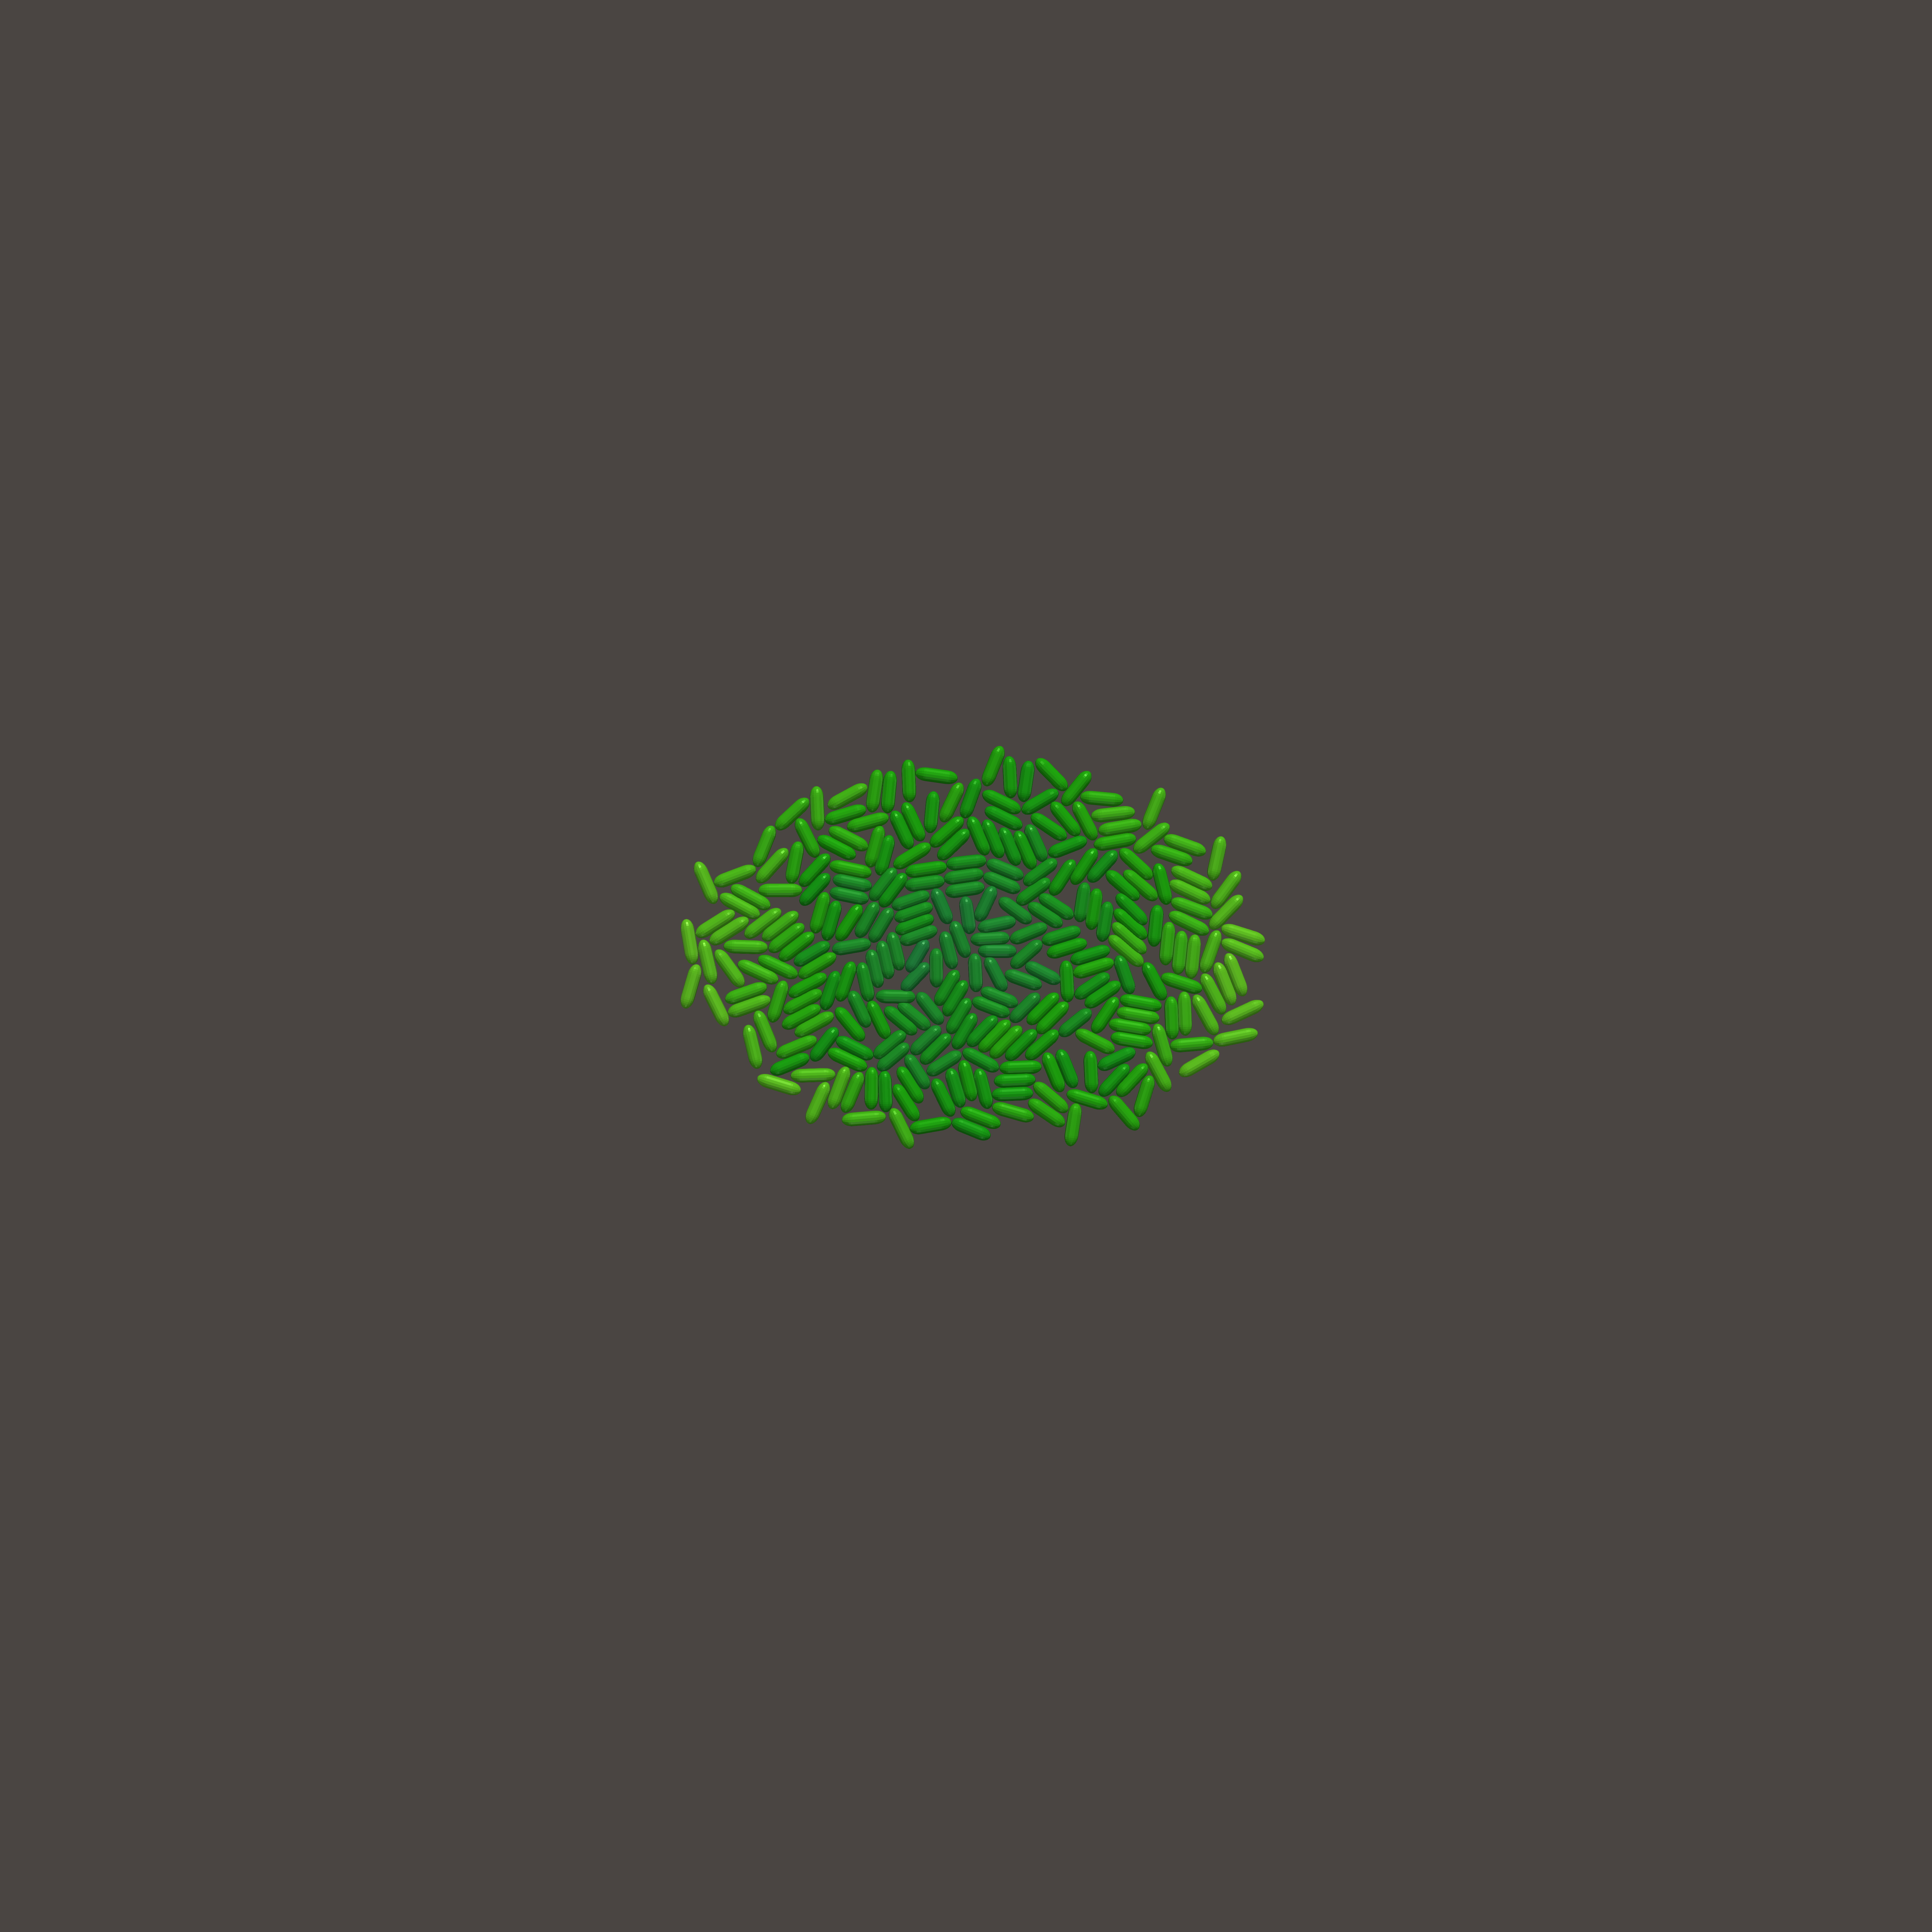
\includegraphics[width=\textwidth]{figures/growth_comparison_lambda_1e-2/soft.0060.png}
            \end{subfigure} &
            \begin{subfigure}[b]{\subfigwidth}
                \includegraphics[width=\textwidth]{figures/growth_comparison_lambda_1e-2/soft.0080.png}
            \end{subfigure} &
            \begin{subfigure}[t]{\subfigwidth}
                \includegraphics[width=\textwidth]{figures/growth_comparison_lambda_1e-2/soft.0100.png}
            \end{subfigure}    \\
        \end{tabular}
        \caption{Growth Comparison $\lambda=10^{-2}$}


    \end{subfigure}

    \vspace{1em}

    \caption{Pattern formation under stress-sensitive growth at different time points. Each row shows the evolution for a different value of $\lambda$, demonstrating how the strength of mechanical feedback affects the emerging patterns. Time points are shown as fractions of the total simulation time $T$.}
    \label{fig:pattern_evolution}
\end{figure*}




\begin{itemize}
    \item Concentric ring reproduction
    \item Quantitative metrics
    \item Model comparison
\end{itemize}

\subsection{Computational Performance}
\begin{itemize}
    \item Runtime scaling
    \item Memory efficiency
    \item Parameter sensitivity
\end{itemize}

\section{Discussion}
\subsection{Model Selection Insights}
\begin{itemize}
    \item When constraints are essential
    \item Computational trade-offs
    \item Practical recommendations
\end{itemize}

\subsection{Biological Relevance}
\begin{itemize}
    \item Model assumptions
    \item Connection to reality
    \item Implications for understanding
\end{itemize}

\section{Conclusion}
\begin{itemize}
    \item Validation of constraint-based approach
    \item Methodological contributions
    \item Future research directions
\end{itemize}

\bibliographystyle{IEEEtran}
\bibliography{literature}

\end{document}